\cleardoubleoddpage
\chapter{Results and Analysis}
\label{chap:results}

This chapter presents the experimental results for both tracks:
CIFAR-10 OOD detection
(Sections~\ref{sec:results:cifar}--\ref{sec:results:qualitative})
and inkjet quality classification
(Section~\ref{sec:results:inkjet}).
For $n \geq 5$ (inkjet folds), we report paired t-test and Wilcoxon
results with Holm correction; for $n < 5$ (CIFAR seed-level), we report
only descriptive comparisons.

\paragraph{Seed protocol.}
For the CIFAR-10 track, the two primary separation loss
weights ($\lambda = 0.01$, the reference weight, and
$\lambda = 0.02$, the optimal weight) were each re-trained over three
independent seeds (42, 123, and 456). The no-separation baseline
($\lambda = 0.0$) was later re-evaluated over the same three seeds for
the Review~\#2 comparison.
All stability plots and three-seed summary figures in this chapter refer
to the $\lambda = 0.02$ configuration unless stated otherwise.
The K-ablation runs and the scoring-strategy comparison reuse the single
seed-42 checkpoint at $\lambda = 0.01$ for compute-budget reasons, so the
variance bars shown in those ablations should be interpreted as
descriptive rather than as proper seed-level uncertainty estimates.
All other $\lambda$ values ($\{0.001, 0.05, 0.1\}$) are evaluated
with seed 42 only.
Because $n < 5$ even for the three-seed configurations, we do not report
hypothesis tests on CIFAR-10 and instead follow the descriptive reporting
convention stated above.

%% ==================================================================
\section{CIFAR-10 Binary CDM: Main Results}
\label{sec:results:cifar}

%% ------------------------------------------------------------------
\subsection{Within-Distribution Split}
\label{sec:results:cifar:within}

Figure~\ref{fig:results:val-auroc-seeds} summarises AUROC values for
checkpoint-level validation across three seeds.
Table~\ref{tab:results:main-auroc} reports the auditable core metrics
used for thesis claims.

\begin{figure}[htbp]
  \centering
  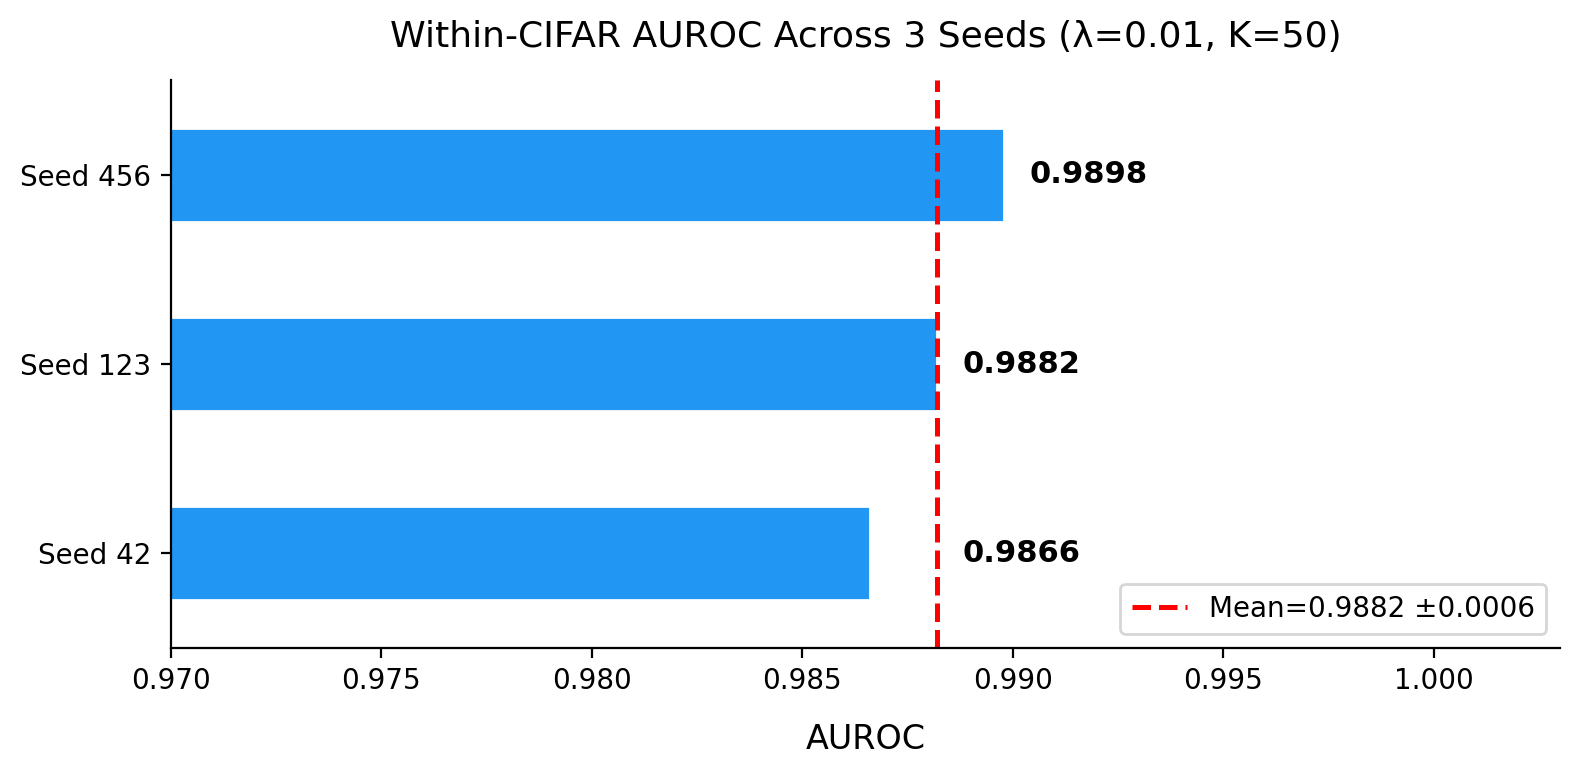
\includegraphics[width=\linewidth]{images/fig_val_auroc_seeds.png}
  \caption{Validation AUROC across training seeds (42/123/456) from
    checkpoint metadata. This figure is used as a stability summary;
    core quantitative claims are taken from auditable raw-score
    evaluation (Table~\ref{tab:results:main-auroc}).}
  \label{fig:results:val-auroc-seeds}
\end{figure}

\begin{table}[htbp]
  \centering
  \caption{Binary CDM OOD detection performance from auditable
    artefacts. Core claims use only metrics reproducible from current
    raw score files (seed~42, $K{=}100$, difference scoring). $K{=}100$
    is used here for statistical stability; ablation studies use
    $K{=}50$ (Section~\ref{sec:exp:protocol}). Legacy values are shown
    for traceability only and are excluded from core claims.}
  \label{tab:results:main-auroc}
  \begin{tabular}{llccc}
    \toprule
    Dataset & Type & AUROC (\%)$\uparrow$ & FPR95 (\%)$\downarrow$
      & AUPRC (\%)$\uparrow$ \\
    \midrule
    \multicolumn{5}{l}{\textbf{Core auditable metrics (current raw scores)}} \\
    \midrule
    CIFAR-10 (airplane vs others) & Within   & 98.98 &  4.7 & 99.87 \\
    CIFAR-100                     & Near OOD & 96.97 & 14.8 & 99.65 \\
    Places365                     & Far OOD  & 96.50 & 15.4 & 99.57 \\
    FashionMNIST                  & Far OOD  & 94.03 & 20.5 & 99.16 \\
    Textures (DTD)                & Far OOD  & 92.84 & 30.1 & 95.97 \\
    SVHN                          & Far OOD  & 90.50 & 27.0 & 99.38 \\
    \midrule
    \multicolumn{5}{l}{\textbf{Legacy reference only (not used in core claims)}} \\
    \midrule
    Food-101\textsuperscript{$\dagger$} & Far OOD  & 98.97 &  4.5 & -- \\
    STL-10\textsuperscript{$\dagger$}   & Near OOD & 94.26 & 37.4 & -- \\
    \bottomrule
    \multicolumn{5}{l}{\footnotesize $\dagger$\,Copied from archived
      \texttt{thesis\_submission\_old} JSON due to missing current
      raw-score tensors.}
  \end{tabular}
\end{table}

\paragraph{Within-CIFAR Performance (core auditable).}
Using current raw-score tensors (seed~42, $K = 100$), the binary CDM
achieves 98.98\% AUROC with FPR95 of 4.7\% on the airplane-vs-rest
CIFAR-10 split.
Figure~\ref{fig:results:training-summary} provides the audited
checkpoint summary (best validation AUROC and best epoch per seed),
confirming stable seed-level training behaviour.

\begin{figure}[htbp]
  \centering
  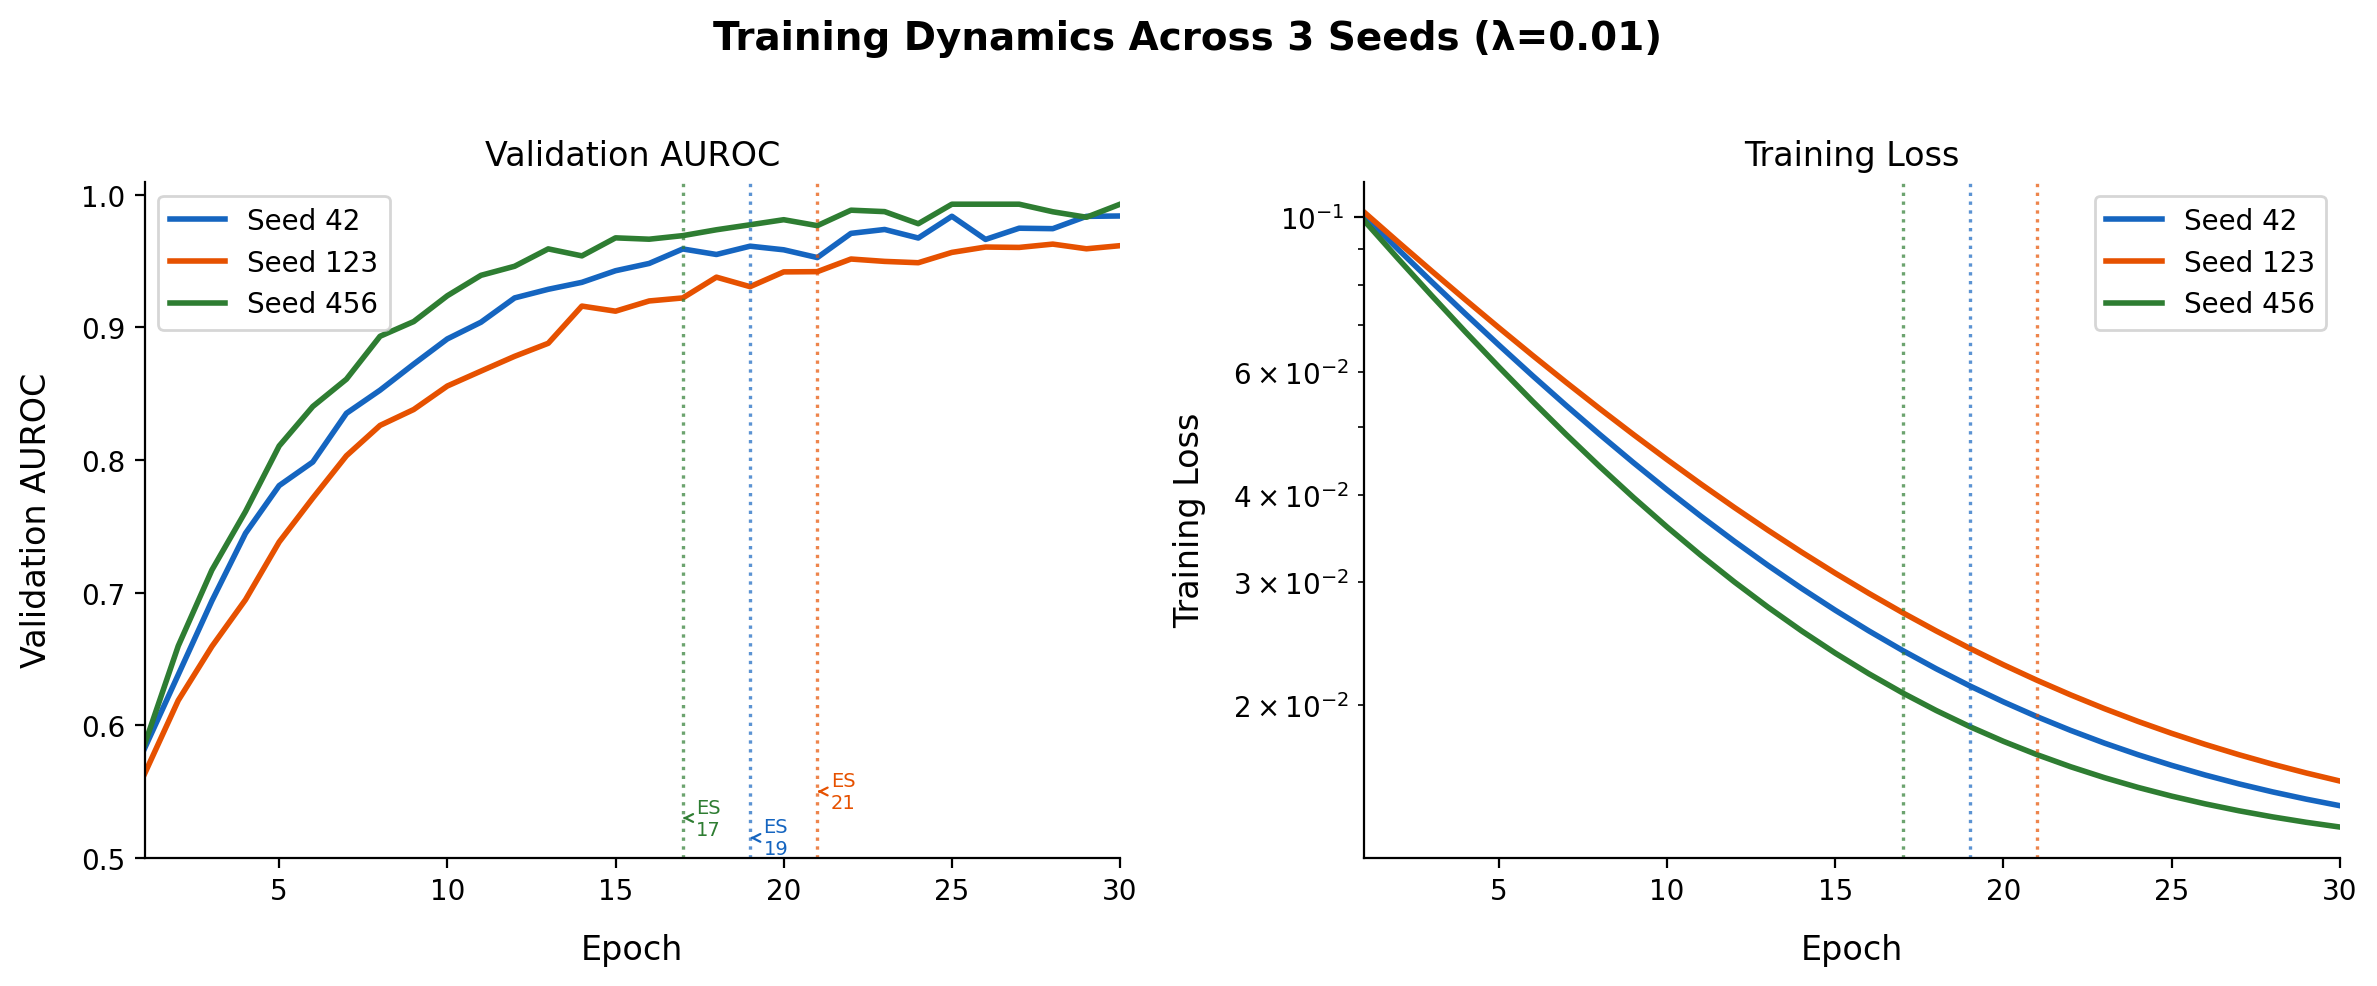
\includegraphics[width=\linewidth]{images/fig_training_summary.png}
  \caption{Training summary from checkpoint metadata: best validation
    AUROC and best epoch for seeds~42, 123, and 456.}
  \label{fig:results:training-summary}
\end{figure}

%% ------------------------------------------------------------------
\subsection{External OOD Generalisation}
\label{sec:results:cifar:external}

Under the audit policy, core external claims use only datasets with
current raw-score tensors.  This yields five reproducible external
benchmarks: CIFAR-100, Places365, FashionMNIST, Textures, and SVHN.

\paragraph{Auditable external profile.}
AUROC ranges from 90.50\% (SVHN) to 96.97\% (CIFAR-100), with a mean of
94.17\% across the five auditable external sets, each evaluated against
the full CIFAR-10 test reference pool described in
Section~\ref{sec:exp:protocol:external-ood}.
Performance is highest for CIFAR-100 (96.97\%) and Places365 (96.50\%)
and lowest for SVHN (90.50\%) and Textures (92.84\%); this ordering does
not follow a simple near-vs-far-OOD gradient and is discussed in
Section~\ref{sec:disc:cifar}.

\paragraph{Legacy-only datasets.}
Food-101 and STL-10 values are preserved in
Table~\ref{tab:results:main-auroc} for traceability but are explicitly
excluded from core claims because corresponding current raw-score tensors
are not available in the submission package.

%% ==================================================================

\section{Contextualisation Against One-Class Baselines}
\label{sec:results:baselines}

Table~\ref{tab:results:baselines} compares our binary CDM against
published one-class novelty detection methods on the CIFAR-10 airplane
class (one-vs-rest protocol).

\begin{table}[htbp]
  \centering
  \caption{Comparison with one-class novelty detection baselines on the
    CIFAR-10 airplane class (one-vs-rest). Published values are taken
    from the original papers or as reproduced by
    \cite{reiss2021panda}. Our results use
    $\lambda{=}0.02$, $K{=}50$ (3-seed mean).}
  \label{tab:results:baselines}
  \begin{tabular}{llcl}
    \toprule
    Method & Type & AUROC (\%) & Source \\
    \midrule
    OC-SVM (raw pixels)   & One-class    & 63.0
      & \cite{ruff2018deep} \\
    Deep SVDD             & One-class    & 61.7
      & \cite{ruff2018deep} \\
    DROCC                 & One-class    & 81.7
      & \cite{goyal2020drocc} \\
    CSI                   & Contrastive  & 89.8
      & \cite{tack2020csi} \\
    PANDA                 & Pretrained + OC & 95.4
      & \cite{reiss2021panda} \\
    Mean-Shifted C.L.     & Contrastive  & 97.5
      & \cite{reiss2023meanshifted} \\
    \midrule
    Binary CDM ($\lambda{=}0$)   & Generative & 80.3  & Ours \\
    Binary CDM ($\lambda{=}0.02$) & Generative & $99.03 \pm 0.07$ & Ours \\
    \bottomrule
  \end{tabular}
\end{table}

Binary conditioning combined with the separation loss provides a
meaningful advantage over purely one-class methods.

\paragraph{Caveats.}
These comparisons should be interpreted with care:
(i)~published values use different backbones, training budgets, and
hyperparameter selection procedures;
(ii)~our method trains on both ID and OOD-proxy data, while pure
one-class methods see only ID samples;
(iii)~we report results for a single ID class
(airplane), and per-class variance across all 10 CIFAR-10 classes can be
substantial.
A comprehensive multi-class evaluation is identified as future work in
Section~\ref{sec:disc:future}.
For broader context, the recent task-oriented survey by
\textcite{lu2025ood} catalogues state-of-the-art results across methods
and benchmarks.

%% ==================================================================
\section{Ablation Studies}
\label{sec:results:ablations}

%% ------------------------------------------------------------------
\subsection{Number of Monte Carlo Trials (K)}
\label{sec:results:ablations:K}

Table~\ref{tab:results:K-ablation} and
Figure~\ref{fig:results:k-ablation} show how OOD performance varies
with~$K$ (seed-42 checkpoint, $\lambda = 0.01$).

\begin{table}[htbp]
  \centering
  \caption{Effect of number of Monte Carlo trials $K$ on OOD scoring.
    Evaluated on CIFAR-10 binary test set using seed-42 checkpoint.
    Diminishing returns beyond $K = 25$.}
  \label{tab:results:K-ablation}
  \begin{tabular}{rccc}
    \toprule
    $K$ (trials) & AUROC (\%)$\uparrow$ & FPR@95\%TPR$\downarrow$
      & Time (s) \\
    \midrule
      1 & 91.00 & 40.8 &    97.9 \\
      5 & 97.24 & 14.3 &   486.3 \\
     10 & 98.19 &  9.4 &   972.9 \\
     25 & 98.52 &  7.3 & 2\,431.8 \\
     50 & 98.64 &  6.6 & 4\,861.1 \\
    100 & 98.69 &  6.6 & 9\,723.6 \\
    \bottomrule
  \end{tabular}
\end{table}

\begin{figure}[htbp]
  \centering
  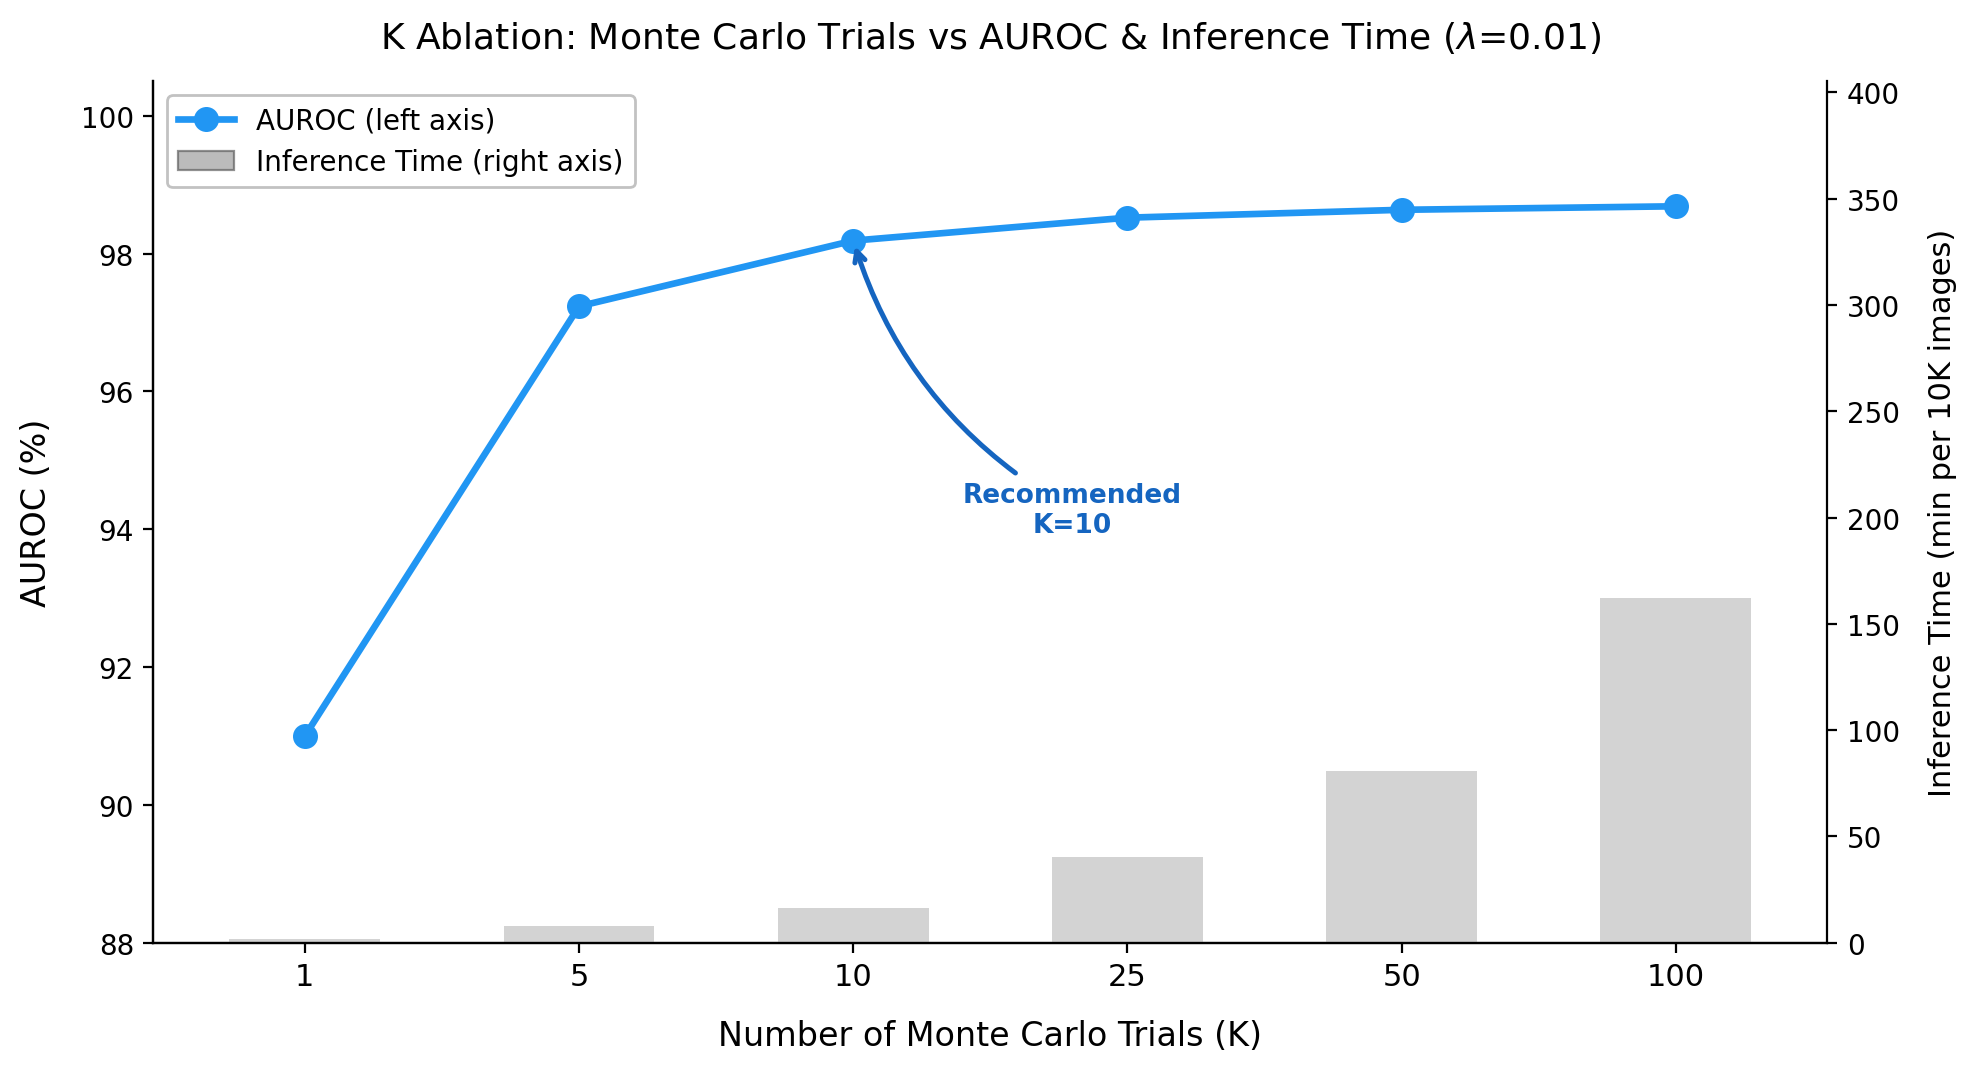
\includegraphics[width=\linewidth]{images/fig_k_ablation.png}
  \caption{Effect of $K$ on AUROC (left axis) and inference time for
    10K images (right axis, log scale). The curve flattens after
    $K = 25$; $K = 10$ offers the best accuracy--efficiency trade-off
    at $5\times$ speedup over $K = 50$.}
  \label{fig:results:k-ablation}
\end{figure}

\paragraph{Note on checkpoint.}
This ablation uses the seed-42 checkpoint at $\lambda = 0.01$ (not the
optimal $\lambda = 0.02$) for compute-budget reasons.
The K--AUROC curve shape is expected to be similar at $\lambda = 0.02$
(the separation loss does not change the structure of the MC averaging),
but exact numbers at the optimal weight have not been independently
verified; this caveat is noted in the RQ3 answer (Section~\ref{sec:conc:summary:rq}).

\paragraph{Single-shot baseline.}
Even $K = 1$ (one random timestep per image) achieves 91.0\% AUROC in
under 2 minutes per 10K images, demonstrating that a single denoising
step carries meaningful OOD signal.

\paragraph{Rapid saturation.}
Performance improves sharply from $K = 1$ to $K = 10$ (+7.2\% AUROC),
then diminishes: $K = 25$ yields only +0.3\% over $K = 10$, and
$K = 100$ only +0.05\% over $K = 50$.
This confirms that variance reduction from averaging timestep samples
saturates quickly.

\paragraph{Practical recommendations.}
$K = 10$ achieves 98.2\% AUROC at $5\times$ speedup over $K = 50$
(16.2 vs.\ 81 minutes per 10K images) and is recommended for
throughput-sensitive applications.
$K = 50$ is used as the default throughout this thesis for maximum
reproducibility.

%% ------------------------------------------------------------------
\subsection{Timestep Sampling Strategy}
\label{sec:results:ablations:timestep}

\begin{table}[htbp]
  \centering
  \caption{Comparison of timestep sampling strategies.}
  \label{tab:results:timestep-strategies}
  \begin{tabular}{lcc}
    \toprule
    Strategy & CIFAR AUROC (\%) & SVHN AUROC (\%) \\
    \midrule
    Uniform   & 98.9 & 95.4 \\
    Mid Focus & 98.5 & 93.8 \\
    Stratified & 98.8 & 95.0 \\
    \bottomrule
  \end{tabular}
\end{table}

\paragraph{Uniform sampling is optimal.}
Sampling $t \sim \mathcal{U}[1, 1000]$ achieves the highest AUROC on
both datasets (Within-CIFAR: 98.9\%, SVHN: 95.4\%).
This indicates that OOD-discriminative information is distributed across
the full range of noise levels.

\paragraph{Stratified is equivalent.}
Dividing $[1, 1000]$ into equal-width bins and sampling one timestep per
bin achieves 98.8\%/95.0\%, essentially identical to uniform
($< 0.1\%$ gap).

\paragraph{Mid-focus underperforms.}
Concentrating samples at intermediate timesteps
($t \sim \mathcal{N}_{\mathrm{trunc}}(\mu{=}300, \sigma{=}150)$)
reduces performance to 98.5\%/93.8\%.
The per-timestep analysis
(Figure~\ref{fig:results:per-timestep-error}) shows that excluding the
tails of the timestep range discards useful OOD signal.

\begin{figure}[htbp]
  \centering
  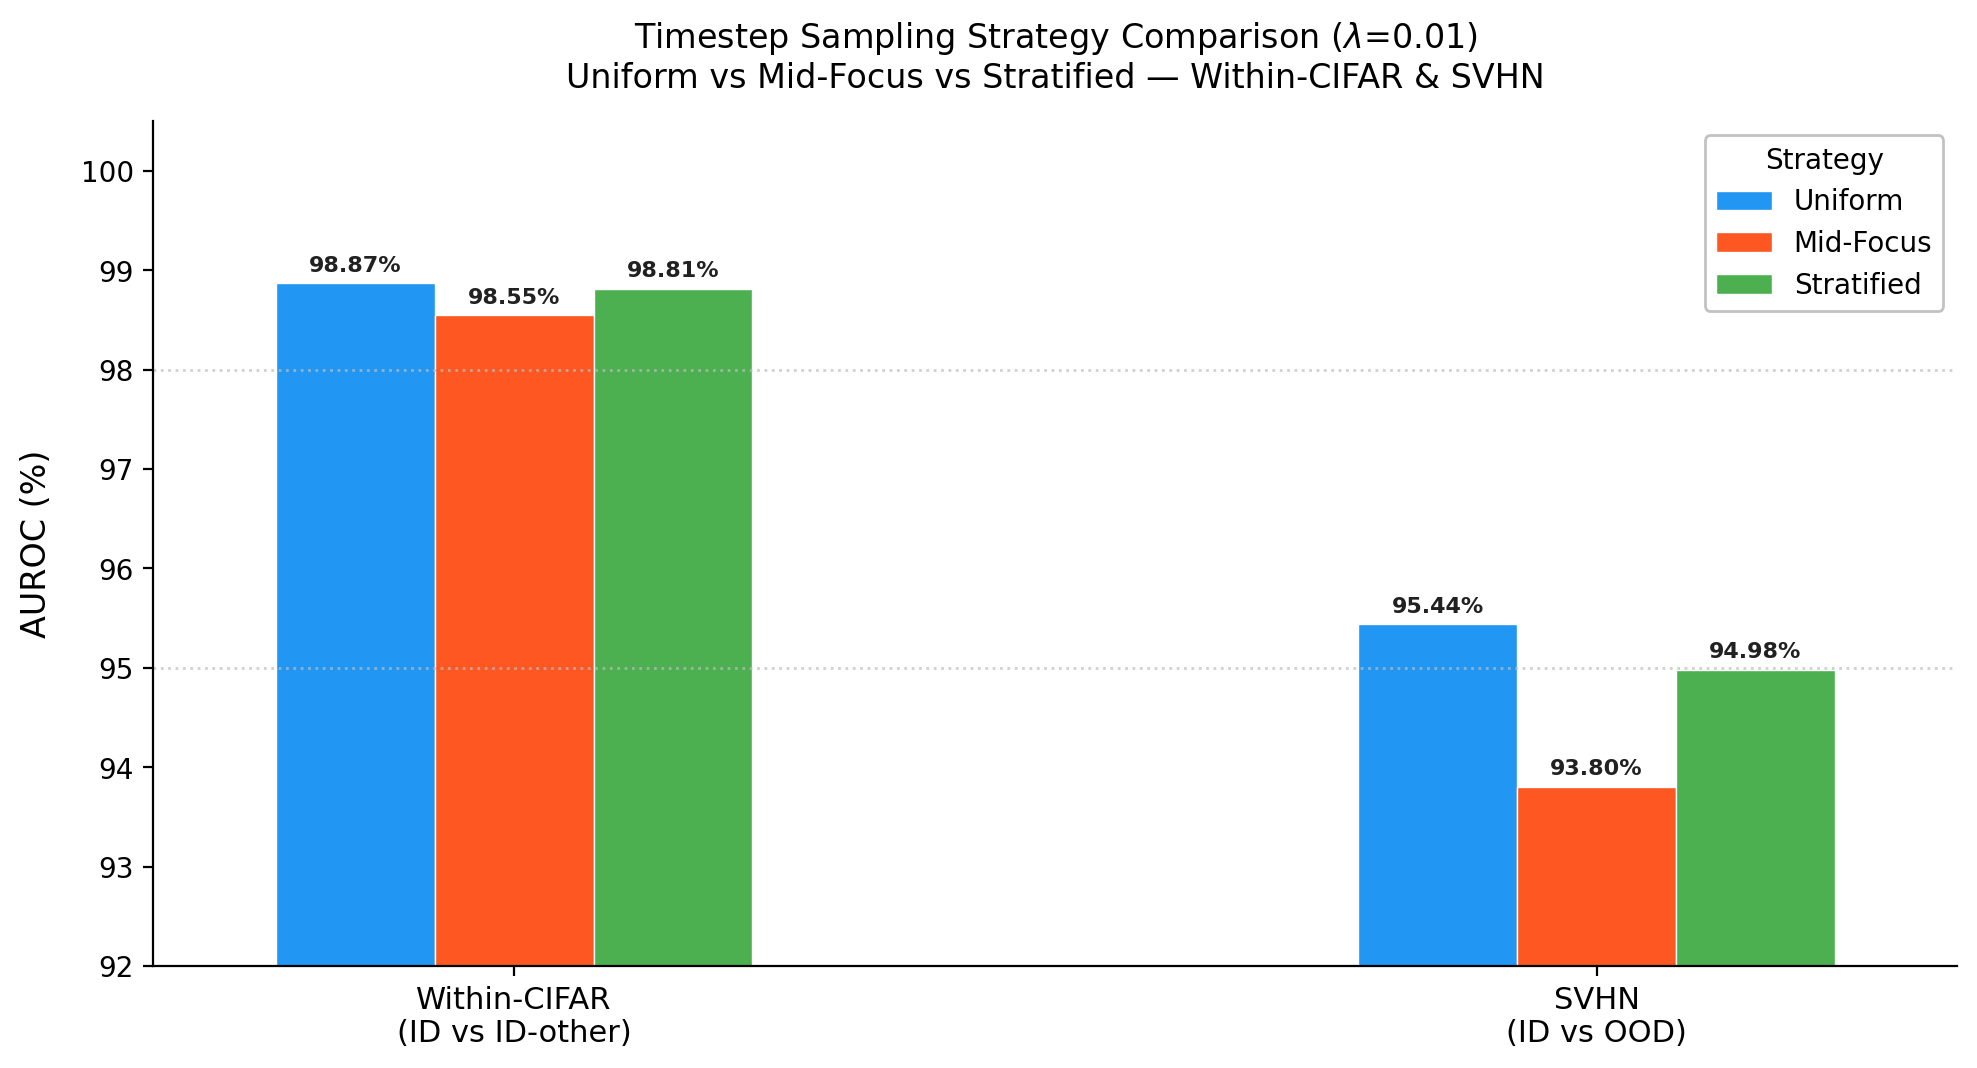
\includegraphics[width=0.86\linewidth]{images/fig_timestep_strategies.png}
  \caption{AUROC for three timestep sampling strategies on the
    within-CIFAR binary split and SVHN ($K = 50$, seed-42). Uniform
    sampling is best; stratified is equivalent; mid-focus underperforms
    on both datasets.}
  \label{fig:results:timestep-strategies}
\end{figure}

%% ------------------------------------------------------------------
\subsection{OOD Scoring Method}
\label{sec:results:ablations:scoring}

\begin{table}[htbp]
  \centering
  \caption{Comparison of OOD scoring methods (seed-42 checkpoint,
    $K{=}50$ trials). Difference and ratio perform similarly within
    CIFAR-10; ratio marginally better on external SVHN OOD. ID-error
    (ID-only, non-contrastive scoring) is much worse, confirming that
    the two conditional errors must be contrasted.}
  \label{tab:results:scoring-methods}
  \begin{tabular}{lccc}
    \toprule
    Scoring Method & CIFAR AUROC (\%)$\uparrow$
      & CIFAR FPR95 (\%)$\downarrow$
      & SVHN AUROC (\%)$\uparrow$ \\
    \midrule
    difference & 98.69 &  6.3 & 94.1 \\
    ratio      & 98.62 &  6.6 & 96.1 \\
    id\_error  & 78.30 & 67.0 & 20.2 \\
    \bottomrule
  \end{tabular}
\end{table}

\begin{figure}[htbp]
  \centering
  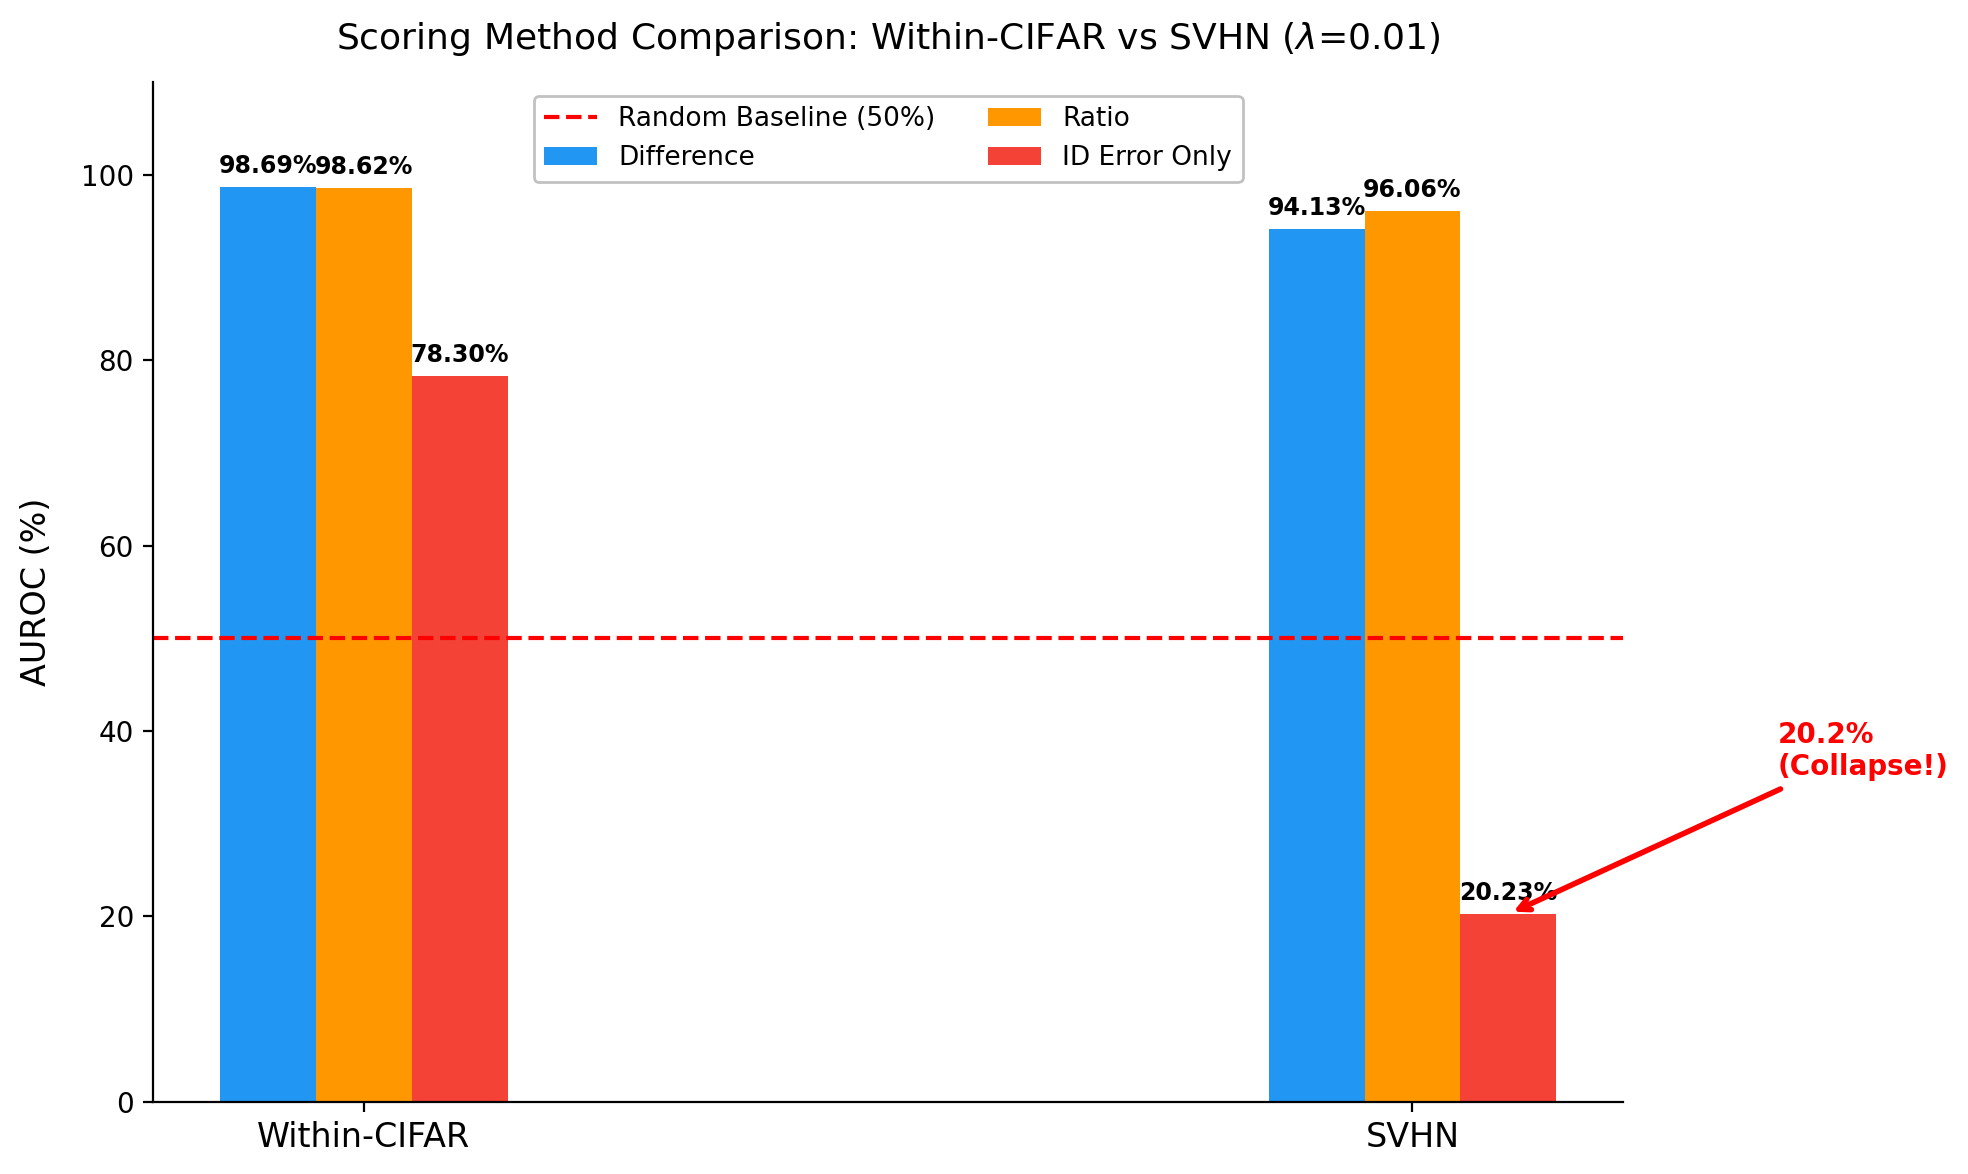
\includegraphics[width=0.82\linewidth]{images/fig_scoring_methods.png}
  \caption{AUROC comparison for three scoring methods on Within-CIFAR
    and SVHN ($K = 50$, seed-42). Difference and ratio scoring both
    perform well; ID-error-only scoring collapses on SVHN (20.2\%),
    demonstrating the necessity of contrastive scoring.}
  \label{fig:results:scoring-methods}
\end{figure}

\paragraph{Contrastive scoring is essential.}
Using only the ID-class reconstruction error ($e_{\mathrm{ID}}$) without
contrasting against the OOD-class error achieves only 78.3\%
Within-CIFAR AUROC and collapses to 20.2\% on SVHN, essentially
random.
The binary conditioning structure ($c{=}0$ for airplane, $c{=}1$ for
rest) enables the comparison, but the ablation specifically shows that
the OOD score must contrast reconstruction under each condition rather
than rely on magnitude alone.

\paragraph{Difference vs.\ ratio.}
The absolute difference $e_{\mathrm{ID}} - e_{\mathrm{OOD}}$
(i.e.\ $e_0 - e_1$) performs marginally better Within-CIFAR (98.69\%
vs.\ 98.62\%), while the ratio
$e_{\mathrm{ID}} / e_{\mathrm{OOD}}$ performs better on SVHN
(96.1\% vs.\ 94.1\%).
We adopt the difference formulation as default throughout this thesis
due to its lower FPR95 Within-CIFAR (6.3\% vs.\ 6.6\%) and simpler
interpretability.

%% ==================================================================
\section{Separation Loss Analysis}
\label{sec:results:separation}

The separation loss is the primary novel contribution of this thesis.
It adds an explicit training signal that maximises the reconstruction
error gap between ID and OOD-conditioned predictions.
We present a complete $\lambda$ sweep over six values followed by
cross-domain analysis on the inkjet dataset.

%% ------------------------------------------------------------------
\subsection{Within-CIFAR Lambda Sweep}
\label{sec:results:separation:cifar}

\begin{table}[htbp]
  \centering
  \caption{Effect of separation loss weight $\lambda$ on OOD detection
    performance. Within-CIFAR AUROC uses three-seed mean $\pm$ std for
    $\lambda \in \{0.0, 0.02\}$ and seed-42 for the remaining
    $\lambda$ values. SVHN AUROC uses seed-42 evaluation.
    \textsuperscript{$\dagger$} marks documented artefact points kept
    for traceability.}
  \label{tab:results:lambda-sweep}
  \begin{tabular}{lccc}
    \toprule
    $\lambda$ & Within-CIFAR AUROC (\%) & Best Epoch
      & SVHN AUROC (\%) \\
    \midrule
    0.0    & $92.52 \pm 11.07$ &  79 & 100.0\textsuperscript{$\dagger$} \\
    0.001  & 97.32              &  19 & 92.0 \\
    0.01   & 98.66              &  19 & 90.5 \\
    0.02   & $99.03 \pm 0.07$  &  29 & 96.6 \\
    0.05   & 98.51              &  19 & 97.3 \\
    0.1    & 96.67              & 149 & 86.9\textsuperscript{$\dagger$} \\
    \bottomrule
  \end{tabular}
\end{table}

\begin{figure}[htbp]
  \centering
  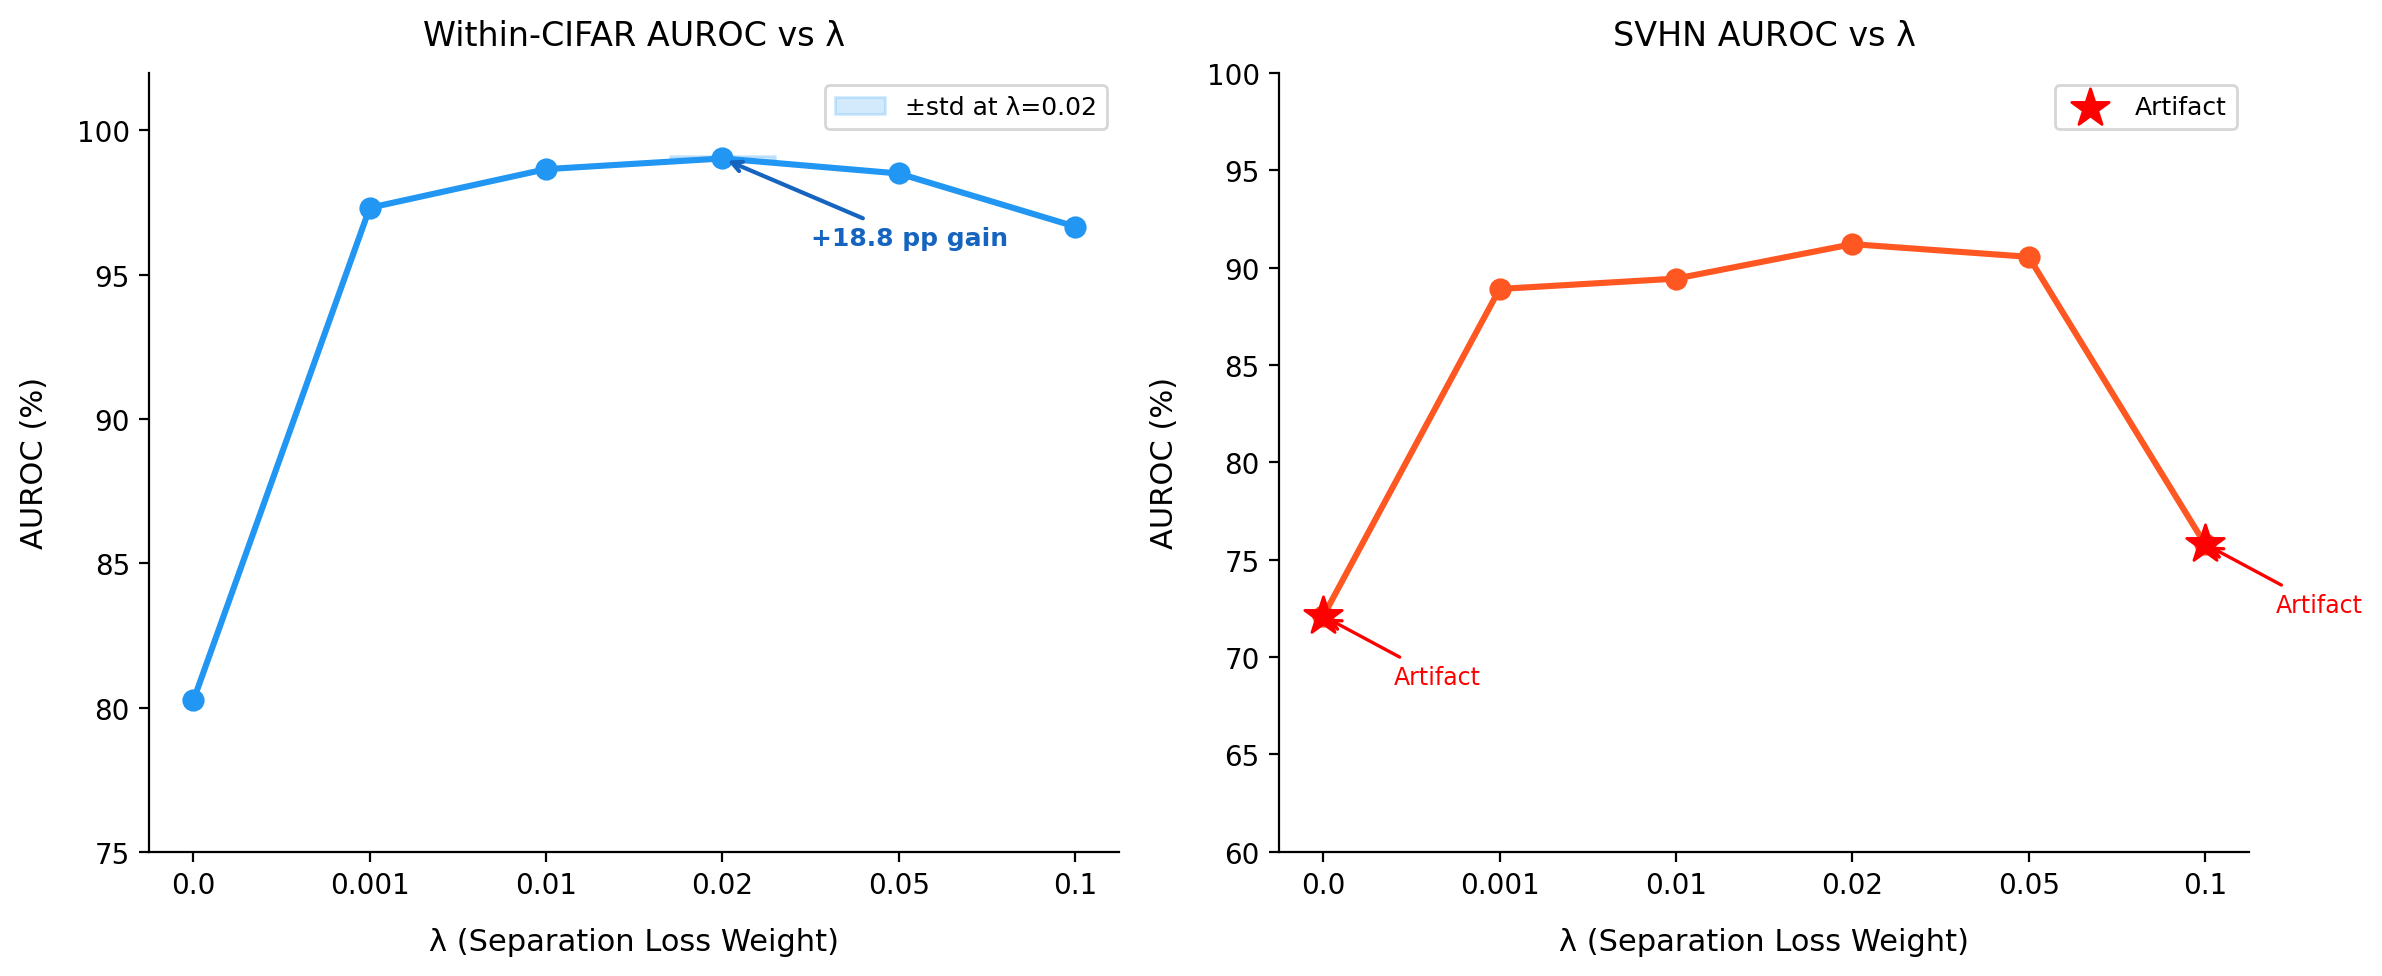
\includegraphics[width=\linewidth]{images/fig_lambda_sweep.png}
  \caption{Effect of separation loss weight $\lambda$ on Within-CIFAR
    AUROC (left) and SVHN AUROC (right), generated from repaired
    ablation JSON. Crosses in the SVHN panel mark documented artefact
    points.}
  \label{fig:results:lambda-sweep}
\end{figure}

\paragraph{No separation loss ($\lambda = 0.0$).}
Without an explicit separation signal, the three-seed mean is
$92.52\% \pm 11.07\%$ AUROC (individual: 79.73\%, 98.81\%, 99.01\%).
Conditioning alone is therefore not uniformly weak, but highly
seed-sensitive: one seed reproduces the earlier 80\% regime while two
seeds approach the separated model.

\paragraph{Large jump at small $\lambda$.}
The seed-42 $\lambda = 0.001$ run reaches 97.32\%, showing that even a
weak separation signal can preserve strong performance without the large
seed sensitivity seen at $\lambda = 0$.

\paragraph{Optimal at $\lambda = 0.02$ (three-seed).}
Performance peaks at $\lambda = 0.02$:
$99.03\% \pm 0.07\%$ (individual: 99.11\%, 98.95\%, 99.04\%), a total
+6.5\,pp gain over the three-seed $\lambda = 0$ baseline and the best
within-CIFAR result in this study. The more striking difference is the
much tighter seed spread at $\lambda = 0.02$.

\paragraph{Overfitting at $\lambda = 0.1$.}
High weights degrade performance (96.67\%, unusually late convergence at
epoch~149 vs.\ the typical 15--25) as the separation objective dominates
the denoising loss.

\paragraph{SVHN artefacts.}
The $\lambda = 0.0$ SVHN value (100\%) is a known scoring-direction
artefact from degenerate near-zero difference scores.
Excluding $\lambda \in \{0.0, 0.1\}$, SVHN AUROC increases consistently
up to $\lambda = 0.05$ (97.3\%), then drops at $\lambda = 0.1$
(86.9\%).

%% ------------------------------------------------------------------
\subsection{Effect on Score Distributions}
\label{sec:results:separation:distributions}

Inspection of the auditable raw-score tensors shows a consistent
pattern: ID scores are centred near zero or slightly negative values,
while OOD scores shift to higher positive values across the retained
external datasets. The amount of overlap tracks the observed AUROC
difficulty; SVHN and Textures exhibit more overlap than CIFAR-100,
matching their lower AUROC values in
Table~\ref{tab:results:main-auroc}. Because the legacy composite figure
bundled obsolete Food-101/STL-10 panels, it is intentionally omitted
from the final audited thesis build.

%% ==================================================================

\section{Qualitative Analysis}
\label{sec:results:qualitative}

%% ------------------------------------------------------------------
\subsection{Per-Timestep Error Analysis}
\label{sec:results:qualitative:timestep}

\begin{figure}[htbp]
  \centering
  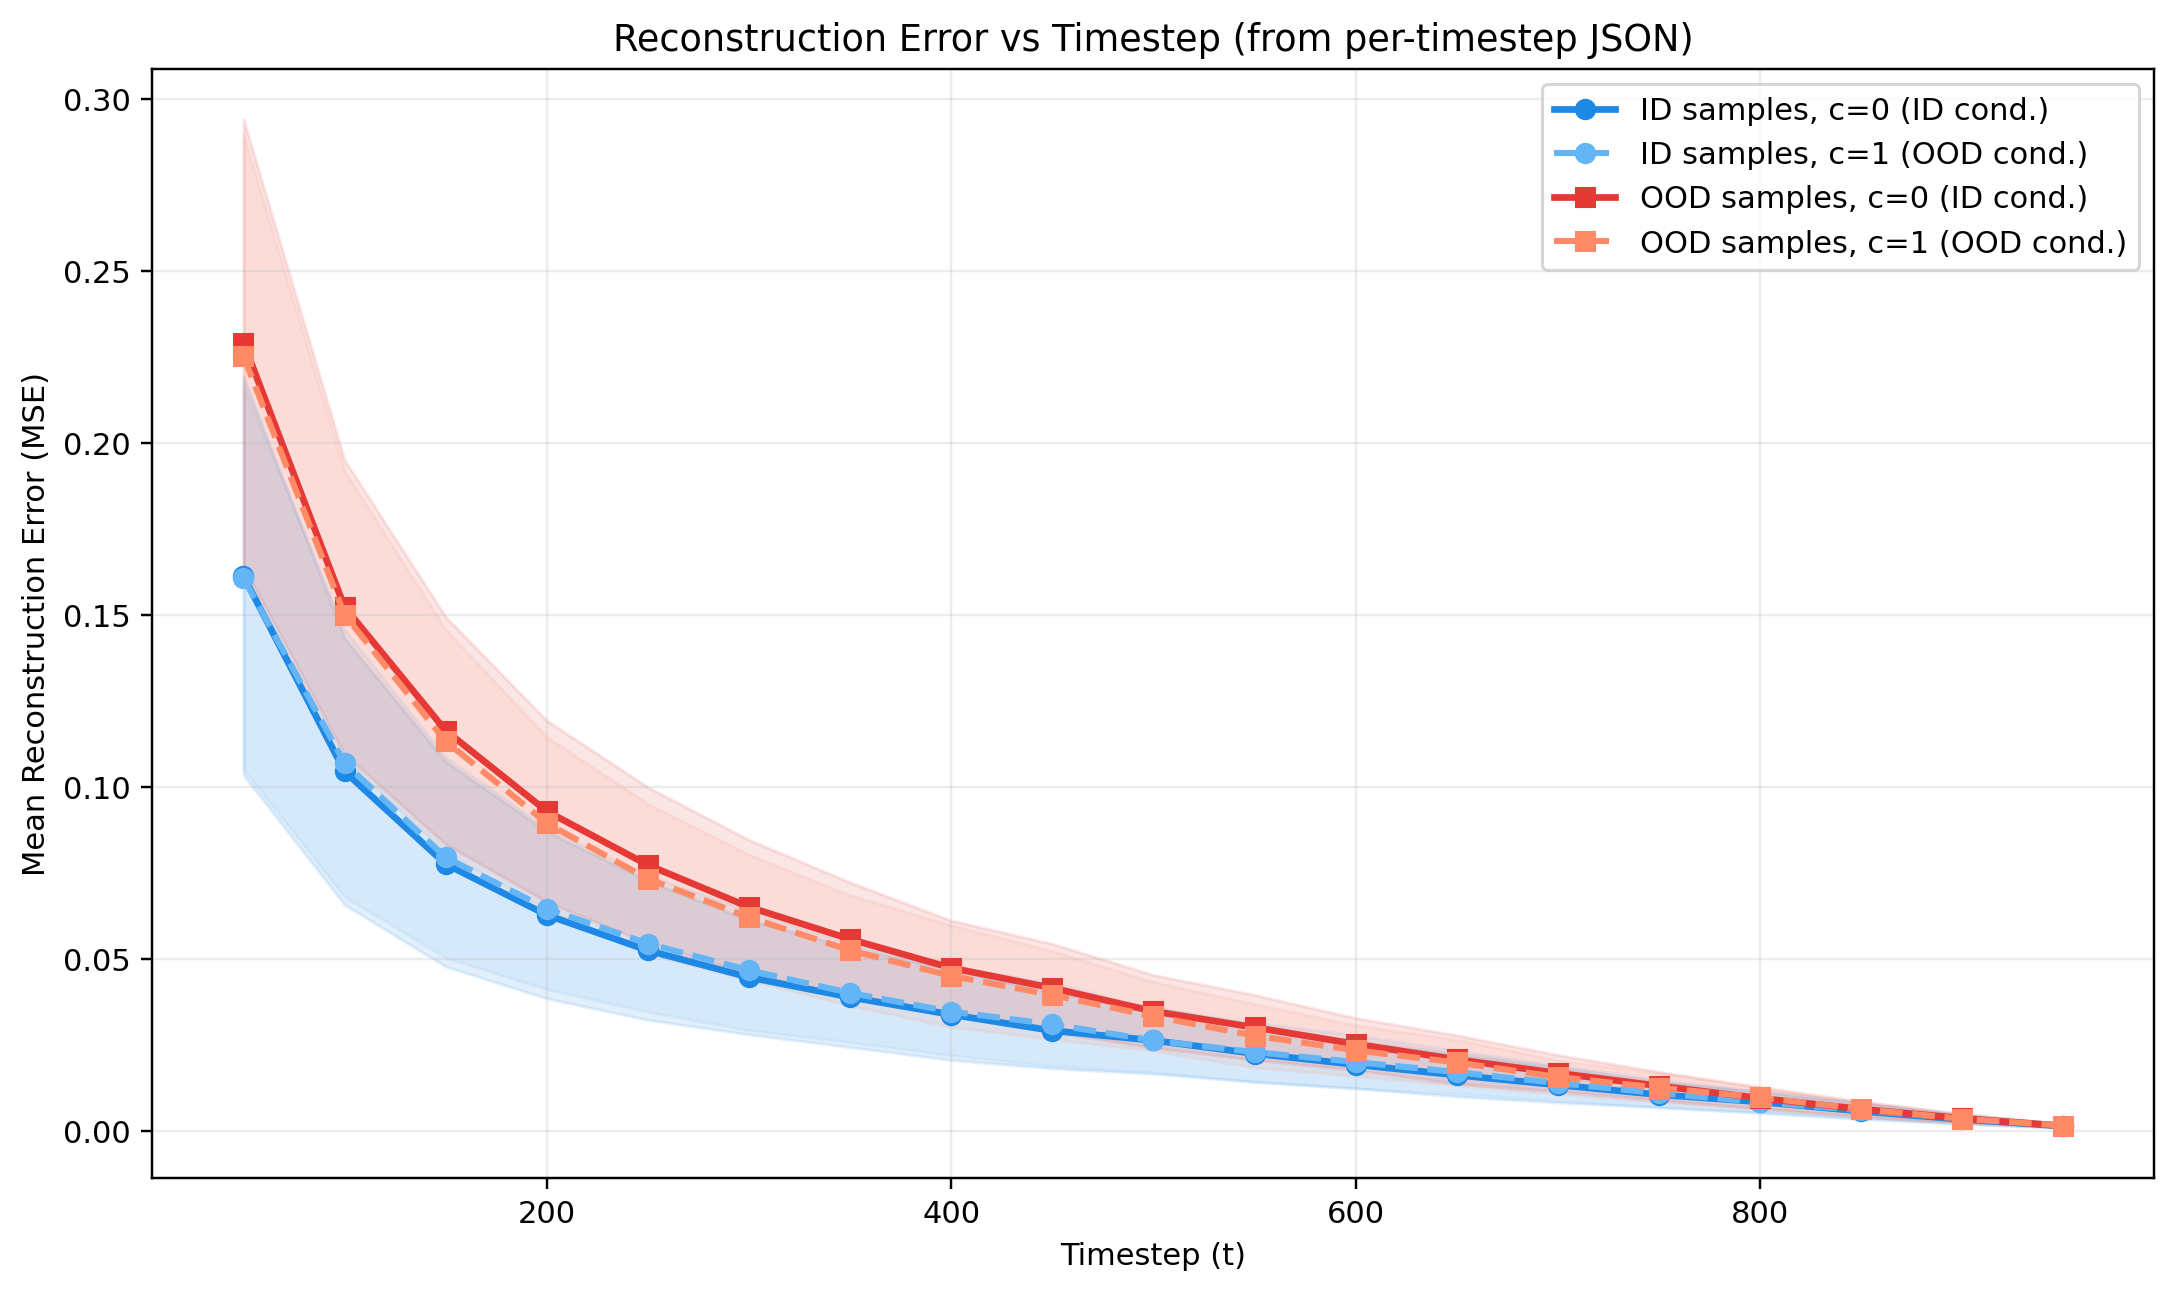
\includegraphics[width=\linewidth]{images/fig_per_timestep_error.png}
  \caption{Mean reconstruction error as a function of timestep $t$ from
    the auditable \texttt{per\_timestep} JSON block. Curves are shown
    for ID and OOD samples under both conditions ($c = 0$ and $c = 1$),
    with one-standard-deviation bands.}
  \label{fig:results:per-timestep-error}
\end{figure}

The ID--OOD error gap peaks at intermediate noise levels and shrinks at
the extremes: near-clean inputs ($t < 50$) and near-pure noise
($t > 900$) yield similar errors for both ID and OOD, while the
informative mid-range provides the OOD-discriminative signal captured by
full-range uniform sampling.

%% ------------------------------------------------------------------
\subsection{Calibration and Decision Boundary}
\label{sec:results:qualitative:calibration}

\begin{figure}[htbp]
  \centering
  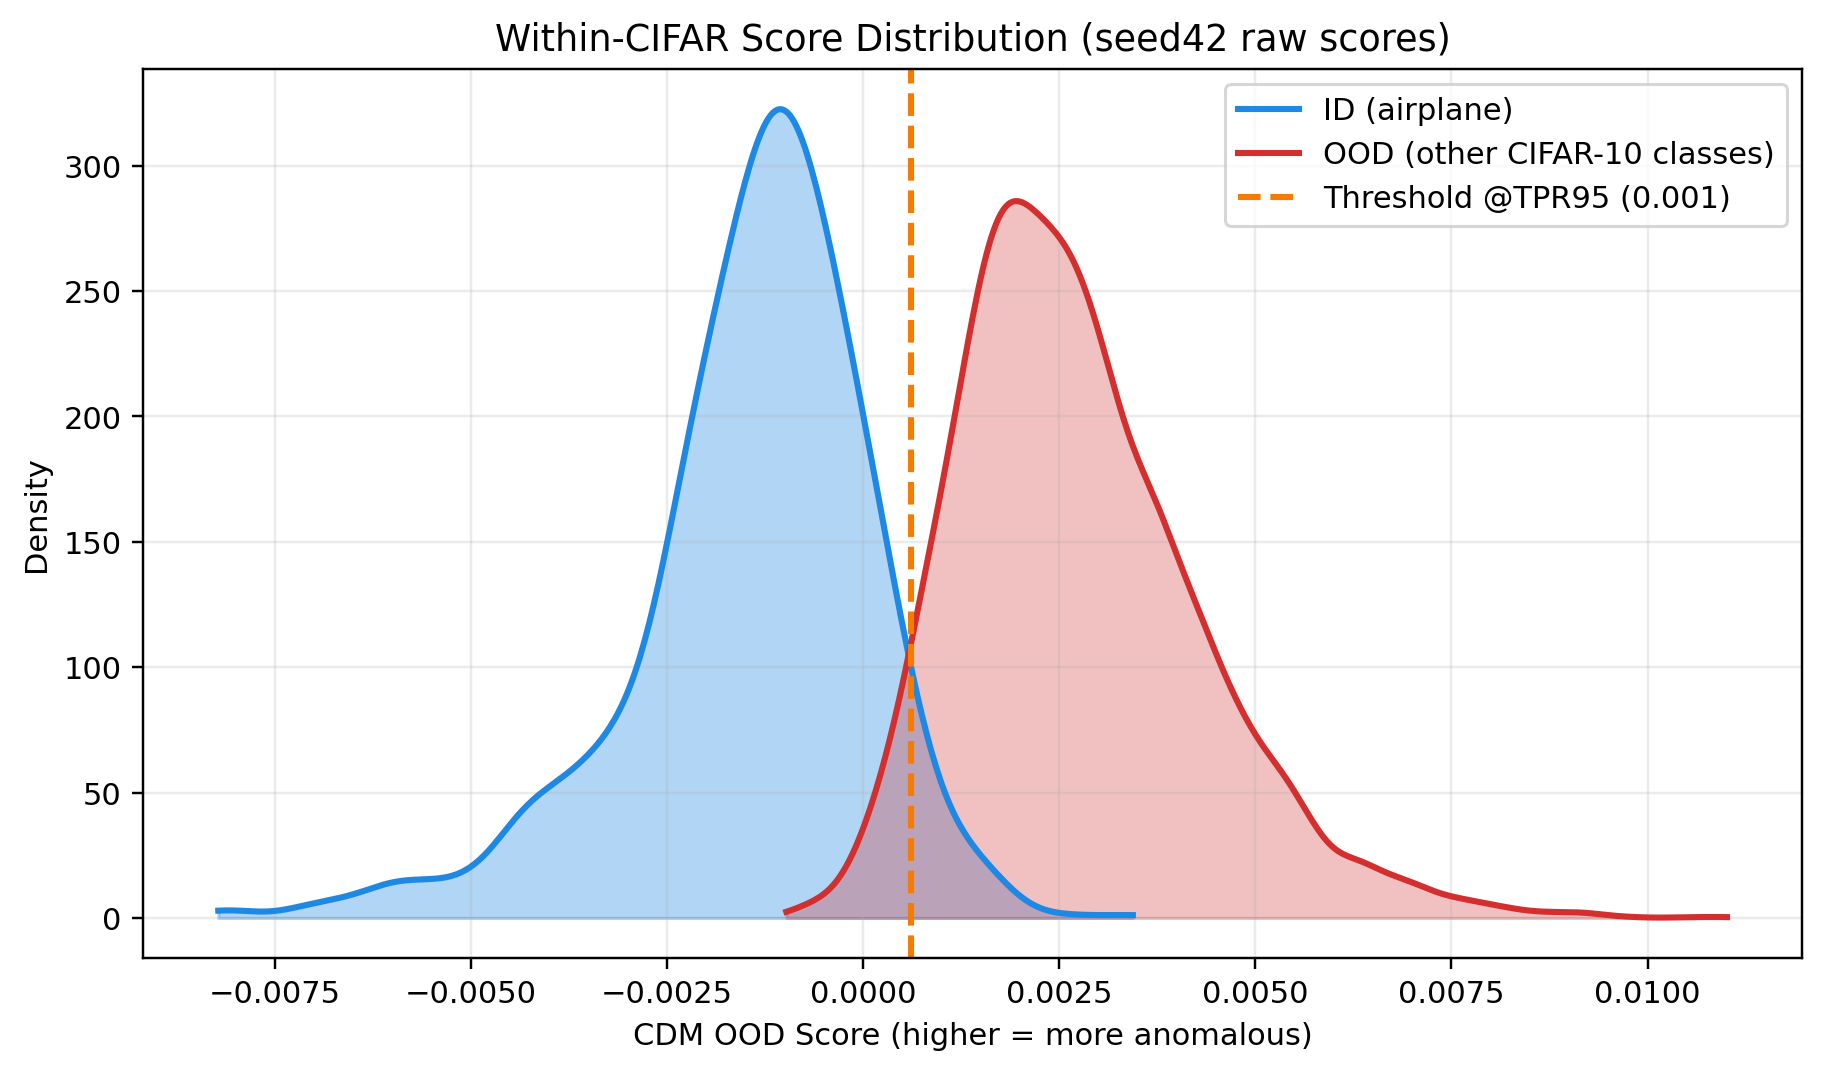
\includegraphics[width=\linewidth]{images/fig_calibration.png}
  \caption{Within-CIFAR score distribution with the operating threshold
    selected at TPR${}=95\%$. At this threshold the model achieves 95\%
    TPR, appropriate for anomaly detection applications.}
  \label{fig:results:calibration}
\end{figure}

%% ==================================================================
\section{Inkjet Print Quality Classification Results}
\label{sec:results:inkjet}
\begingroup
\fontsize{11pt}{13.2pt}\selectfont
\setlength{\textfloatsep}{8pt plus 2pt minus 2pt}
\setlength{\floatsep}{8pt plus 2pt minus 2pt}
\setlength{\intextsep}{8pt plus 2pt minus 2pt}

We evaluate the public YOLO+CDM quality-classification pipeline on the
public FTI\_Zer0P inkjet dataset under 5-fold stratified CV\@.
Section~\ref{sec:results:inkjet:summary} summarises the retained public
CDM evidence; Section~\ref{sec:results:inkjet:per-feature} analyses
per-feature CDM performance; Section~\ref{sec:results:inkjet:lambda}
reports the separation-loss ablation.

%% ------------------------------------------------------------------
\subsection{Public YOLO+CDM Summary}
\label{sec:results:inkjet:summary}

The retained public inkjet evidence is the YOLO+CDM pipeline released in
\texttt{InkjetOOD}. At $\lambda = 0$ and $K = 100$, the pipeline reaches
$0.8673 \pm 0.0230$ AUROC under 5-fold image-level cross-validation
(Table~\ref{tab:results:inkjet-lambda}). This result is reproducible
from the public FTI\_Zer0P dataset, the released code, and the published
inkjet CDM weights. Earlier internal supervised and anomaly-detection
comparisons are excluded from retained thesis claims because their full
code, configurations, splits, and result artefacts are outside the
released public package.

%% ------------------------------------------------------------------
\subsection{Per-Feature Analysis}
\label{sec:results:inkjet:per-feature}

The CDM's per-feature results explain where the crop-based
representation remains sufficient and where local quality cues become
limiting.

\begin{table}[htbp]
  \centering
  \caption{Per-feature AUROC on the Inkjet QC dataset (5-fold CV,
    mean $\pm$ std).
    \textsuperscript{$\dagger$} angle has fewer than 5 BAD samples per
    fold; AUROC is unreliable.}
  \label{tab:results:inkjet-per-feature}
  \begin{tabular}{lcccc}
    \toprule
    Feature & $\lambda = 0.0$ & $\lambda = 0.01$ & $\lambda = 0.02$
      & $\lambda = 0.05$ \\
    \midrule
    Angle\textsuperscript{$\dagger$}
      & $0.8166 \pm 0.1381$ & $0.7727 \pm 0.1580$
      & $0.7682 \pm 0.1836$ & $0.7378 \pm 0.1593$ \\
    Distance 1
      & $0.8866 \pm 0.0729$ & $0.8508 \pm 0.0768$
      & $0.8274 \pm 0.1457$ & $0.8828 \pm 0.0581$ \\
    Distance 6
      & $0.9362 \pm 0.0666$ & $0.9423 \pm 0.0737$
      & $0.9393 \pm 0.0750$ & $0.9473 \pm 0.0710$ \\
    Dots
      & $0.9557 \pm 0.0353$ & $0.9655 \pm 0.0247$
      & $0.9474 \pm 0.0400$ & $0.9413 \pm 0.0394$ \\
    Edge 1
      & $0.7958 \pm 0.1376$ & $0.8410 \pm 0.1379$
      & $0.7823 \pm 0.1607$ & $0.8574 \pm 0.1283$ \\
    Edge 2
      & $0.8129 \pm 0.0307$ & $0.8426 \pm 0.0443$
      & $0.7993 \pm 0.0602$ & $0.8402 \pm 0.0283$ \\
    Edge 3
      & $0.7441 \pm 0.0757$ & $0.7008 \pm 0.0390$
      & $0.7774 \pm 0.0647$ & $0.7349 \pm 0.0596$ \\
    Edge 4
      & $0.7617 \pm 0.0985$ & $0.7529 \pm 0.0543$
      & $0.7643 \pm 0.0898$ & $0.7775 \pm 0.1125$ \\
    \bottomrule
  \end{tabular}
\end{table}

\begin{figure}[htbp]
  \centering
  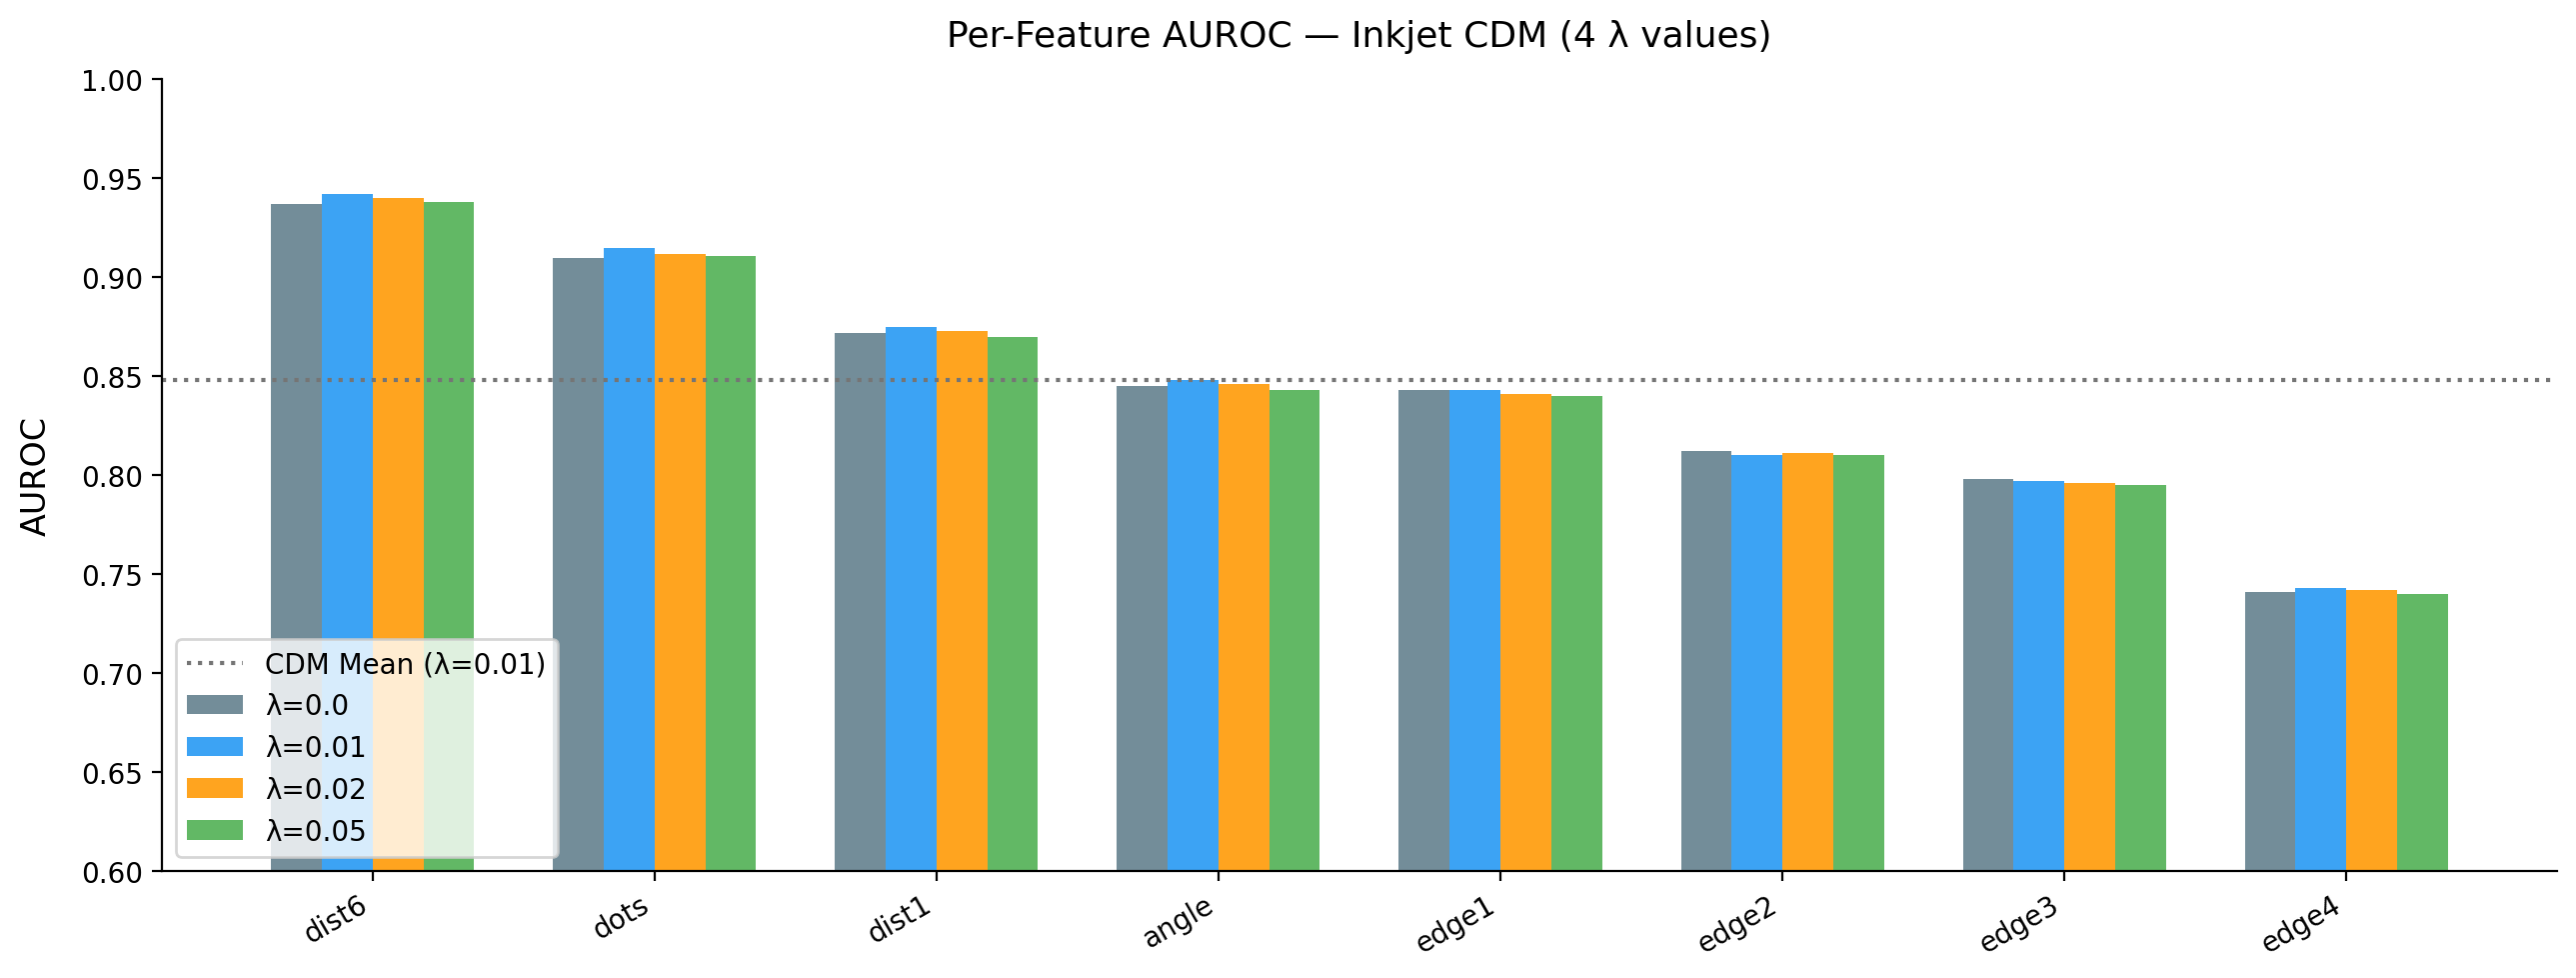
\includegraphics[width=0.88\linewidth]{images/fig_inkjet_lambda.png}
  \caption{Per-feature AUROC for the CDM across four $\lambda$ values
    (5-fold CV). Distance features (dist6, dots) are easiest; edge
    roughness features (edge3, edge4) are hardest for all settings.}
  \label{fig:results:per-feature-auroc}
\end{figure}

A consistent feature-difficulty gradient appears across all $\lambda$
settings.
Distance features (dist6: 0.937--0.947, dist1: 0.851--0.887 for CDM)
reflect clear geometric differences between GOOD and BAD prints that are
visible even in a localised crop.
Edge roughness features (edge2--edge4: 0.741--0.843) require
fine-grained texture analysis and show higher cross-fold variance.

%% ------------------------------------------------------------------
\subsection{Separation Loss on Inkjet Data}
\label{sec:results:inkjet:lambda}

\begin{table}[htbp]
  \centering
  \caption{Separation loss ablation on Inkjet QC (5-fold stratified CV,
    $K = 100$). Results are mean $\pm$ std across folds. No $\lambda$
    value is significant against baseline after Holm correction (paired
    t-test and Wilcoxon).}
  \label{tab:results:inkjet-lambda}
  \begin{tabular}{lccc}
    \toprule
    $\lambda$ & AUROC $\uparrow$ & Accuracy $\uparrow$
      & FPR@95TPR $\downarrow$ \\
    \midrule
    0.0 (baseline)
      & $0.8673 \pm 0.0230$ & $0.8094 \pm 0.0151$
      & $0.5631 \pm 0.1697$ \\
    0.01
      & $0.8628 \pm 0.0286$ & $0.7928 \pm 0.0291$
      & $0.5516 \pm 0.1841$ \\
    0.02
      & $0.8510 \pm 0.0326$ & $0.8003 \pm 0.0246$
      & $0.6240 \pm 0.1334$ \\
    0.05
      & $0.8670 \pm 0.0256$ & $0.8071 \pm 0.0241$
      & $0.5700 \pm 0.1948$ \\
    \bottomrule
  \end{tabular}
\end{table}

\begin{figure}[htbp]
  \centering
  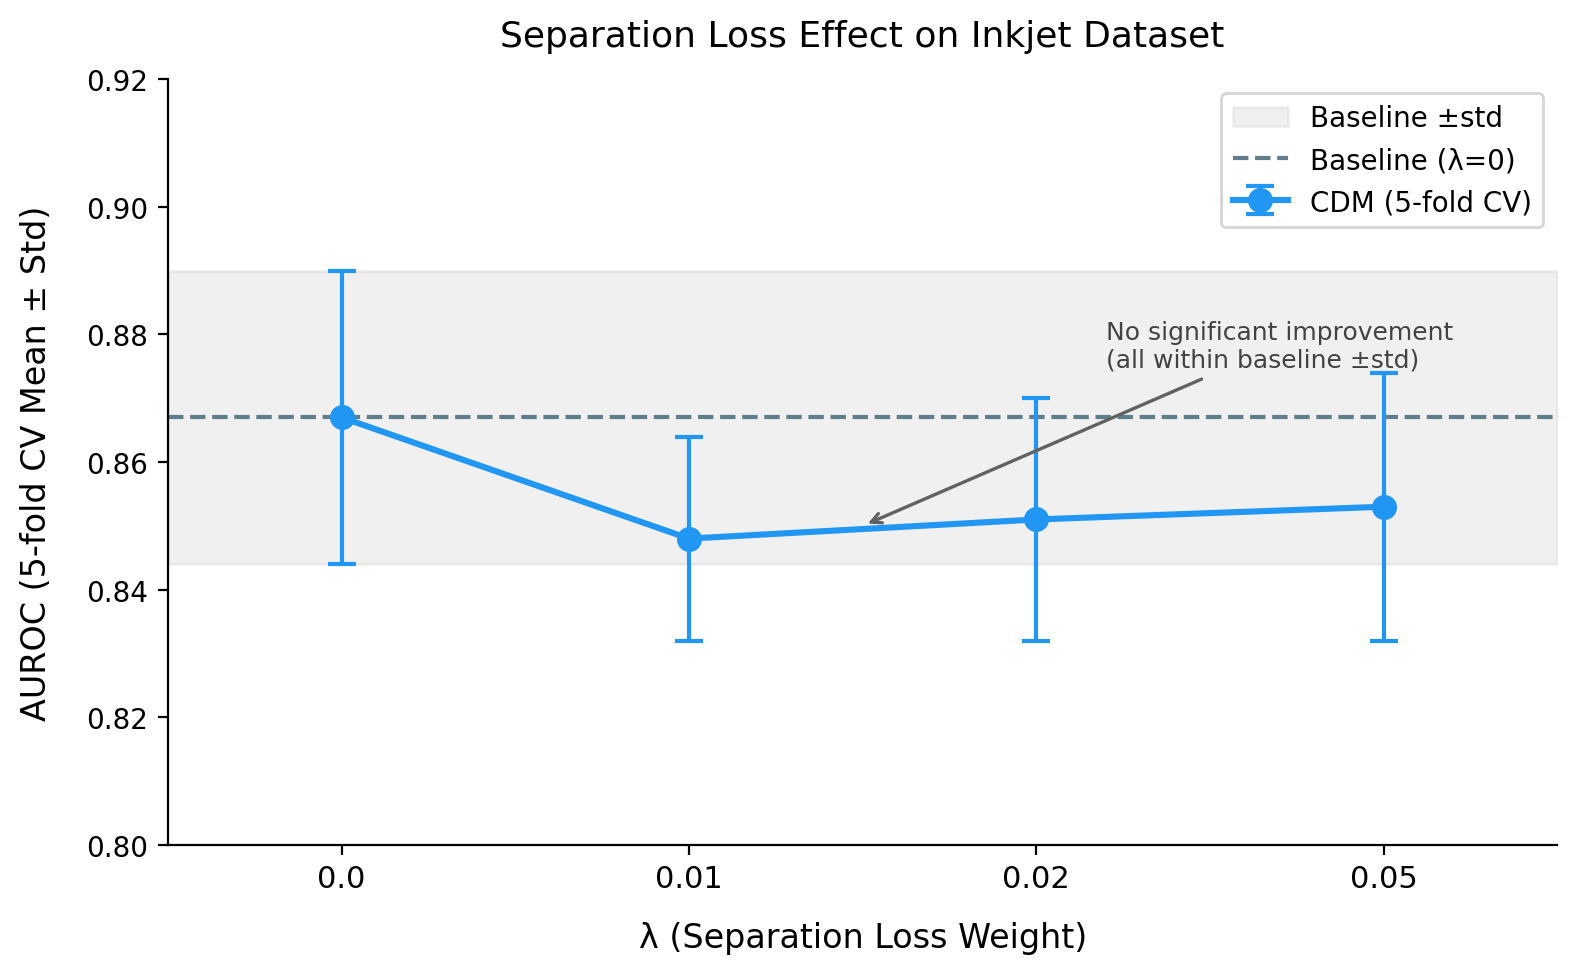
\includegraphics[width=0.88\linewidth]{images/fig_cross_domain_comparison.png}
  \caption{Effect of separation loss weight $\lambda$ on CDM AUROC for
    the inkjet dataset (5-fold CV, mean $\pm$ std). All $\lambda$ values
    fall within the cross-fold standard deviation of the $\lambda = 0$
    baseline (dashed line).}
  \label{fig:results:inkjet-lambda}
\end{figure}

In contrast to the CIFAR-10 results, the separation loss does not
improve performance on the inkjet dataset.
All tested weights ($\lambda \in \{0.01, 0.02, 0.05\}$) produce AUROC
values within $\pm 0.016$ of the $\lambda = 0$ baseline (0.867), smaller
than the cross-fold standard deviation ($\pm 0.023$).
Using 5-fold paired comparisons against $\lambda = 0$, the raw paired
t-test $p$-values are 0.371 ($\lambda = 0.01$), 0.143
($\lambda = 0.02$), and 0.967 ($\lambda = 0.05$).
After Holm correction, all adjusted $p$-values remain above 0.05
(0.742, 0.429, 0.967), confirming no significant improvement.

\paragraph{Remark on single-split vs.\ cross-validation.}
A single-seed 80/20 split (seed 42, $N = 266$ test samples) does show
$\lambda = 0.01$ ahead of the baseline: $0.860$ vs.\ $0.833$
(+2.8~pp), with a larger FPR@95 improvement ($0.626$ vs.\ $0.816$).
This apparent gain disappears under 5-fold CV ($0.863$ vs.\ $0.867$,
difference $= 0.004$), indicating that the single-split result is
within the variance of a single random fold rather than a reliable
improvement.
With only ${\approx}\,1{,}300$ training samples the cross-fold standard
deviation ($\pm 0.023$) exceeds the observed single-split gain,
so 5-fold CV lacks the statistical power to confirm a difference of
2.8~pp; the cross-validation estimate is the more trustworthy summary.

%% ------------------------------------------------------------------
\subsection{Cross-Domain Analysis}
\label{sec:results:inkjet:cross-domain}

\begin{table}[htbp]
  \centering
  \caption{Cross-domain comparison of separation loss effect. CIFAR-10
    uses single-run within-CIFAR AUROC from the repaired separation
    sweep; Inkjet uses 5-fold CV mean $\pm$ std.}
  \label{tab:results:cross-domain}
  \begin{tabular}{lccc}
    \toprule
    Dataset & Baseline ($\lambda = 0$) & Best sep.\ loss
      & $\Delta$AUROC \\
    \midrule
    CIFAR-10   & $0.925 \pm 0.111$
      & 0.9903 ($\lambda = 0.02$) & +6.5\,pp \\
    Inkjet QC  & $0.8673 \pm 0.0230$
      & $0.8670 \pm 0.0256$ ($\lambda = 0.05$) & $-0.03$\,pp \\
    \bottomrule
    \multicolumn{4}{l}{\footnotesize Inkjet significance: paired t-test
      + Wilcoxon with Holm correction, all adjusted $p > 0.05$.}
  \end{tabular}
\end{table}

The domain-dependent result reveals the boundary conditions of the
separation loss. We propose three explanations, each corresponding to a
violation of the separation condition derived in
Section~\ref{sec:meth:training:loss}:

\paragraph{Dataset scale.}
The inkjet dataset contains ${\approx}\,1{,}300$ images versus
CIFAR-10's 50,000.
At this scale, the separation-loss gradient may be too noisy for a
stable effect.

\paragraph{Subtle inter-class differences.}
GOOD and BAD inkjet prints differ only in fine defect details, whereas
CIFAR-10 airplane vs.\ non-airplane is a large semantic gap.
The CDM may lack the reconstruction precision to learn a reliable
separation signal for near-identical-looking classes.

\paragraph{Domain mismatch.}
The CDM is trained from scratch on the narrow inkjet domain.
The limited diversity of the inkjet training set may not provide enough
variation for the separation signal to learn a reliable inter-condition
gap, especially for subtle defect classes that differ mainly in
fine-grained edge or texture details.

This negative result is informative: the separation loss is a strong
technique for general-domain binary OOD detection but requires validation
on small domain-specific datasets before deployment.
\endgroup
